\documentclass{SSBAtran}
\usepackage{graphicx}
\usepackage[cmex10]{amsmath}


% *** PDF, URL AND HYPERLINK PACKAGES ***
%
%\usepackage{url}
% url.sty was written by Donald Arseneau. It provides better support for
% handling and breaking URLs. url.sty is already installed on most LaTeX
% systems. The latest version can be obtained at:
% http://www.ctan.org/tex-archive/macros/latex/contrib/misc/
% Read the url.sty source comments for usage information. Basically,
% \url{my_url_here}.





% *** Do not adjust lengths that control margins, column widths, etc. ***
% *** Do not use packages that alter fonts (such as pslatex).         ***

\usepackage{color} % For inkscape pdf+latex image import

% correct bad hyphenation here
\hyphenation{op-tical net-works semi-conduc-tor}


\begin{document}
%
% paper title
% can use linebreaks \\ within to get better formatting as desired
\title{Metric scale with non-overlapping cameras\\ the 5+1 point method}

% author names and affiliations

\author{
	\IEEEauthorblockN{ Mikael Persson, Andreas Robinson }
	\IEEEauthorblockA{Computer Vision Laboratory, Link\"oping University\\
		Email: $\{$mikael.persson, andreas.robinson$\}$@liu.se}
}

\maketitle


\begin{abstract}
Although popular in many applications, a monocular setup cannot recover the travel distance or translation scale without the use of contextual information or fusion with other sensors. Stereo provides a simple solution at the cost of two cameras but does so without a corresponding increasing of the field of view. However, under certain motion conditions, scale is observable with a non-overlapping pair of cameras mounted in a rigid frame. This provides the benefit of metric reconstructions and fully exploits the increased field of view across two cameras. We present an implementation of a method for recovering the relative pose including translation scale when such a camera pair is used. We also discuss the degenerate cases and provide a quality measure of the estimated scale.
\end{abstract}
\section{Introduction}
The use of cameras to provide vision-based surround sensing seems intuitively a good idea, likely in part because vision plays such a large role in our perception. Vision-based surround awareness can be achieved many ways which we categorize as: 
\begin{itemize}
\item Mobile sensor 
\item Wide field sensor ie fish-eye/parabolic mirror based. 
\item Multi camera arrays
\end{itemize}
Mobile sensors have famously been used on the mars rovers, but have seen little in general robotics, as they are limited by maneuvering arm performance. Wide field sensors are growing in popularity among researchers, but place strong restrictions on the mount and robot chassis and remain expensive. Using multiple regular cameras is straightforward given the large number of powerful real time monocular structure from motion~(SFM) systems today available today~\cite{engel14eccv,mythesis}. Late fusion, i.e. at the point-cloud / odometry stage, provides a straightforward and simple-to-implement system which, given known extrinsics and sufficient excitation through motion, provides metric reconstructions. In practice there is much to gain from an early fusion, ie at the image correspondence stage, as this makes the associations more robust. This is especially important, due to the approximations used to limit the combinatorial explosion otherwise caused by association-uncertainty propagation inherent to feature point trackers and matchers. One example of a early fusion is the Cv4x NView SFM framework by Persson et al~\cite{persson2015robust}. Cv4x essentially performs a joint odometry estimation for each frame through bootstrap tracking for a rigid camera set. In order to extend Cv4x for the non overlapping case we required an appropriate minimal case solver. \\

In this technical report we discuss the properties of an implementation of a scale estimator equivalent to the work of Clipp et al~\cite{clipp2008robust} used in conjunction with a RANSAC based standard essential-matrix solver. 



\section{Related Work}
In the pinhole camera model, all light rays pass through the image plane and converge on the camera center. If both the image plane and the constraint that all rays pass through a common point are removed, the new camera model is referred to as \textit{generalized}. For some generalized camera configurations it is possible to recover the scale and thus translation distance from six points observed at two instances in time, and several methods have been developed. The general minimal case solver by Stewenius et al uses Gr\"obner basis and results in up to 64 solutions~\cite{stewenius2005solutions}. This theoretically appealing solver comes at the cost of computational efficiency and requires high-precision floating point types. 

Li et al argue that small rotations are likely in many applications and present a method which relies on linearizing the rotation~\cite{li2008linear}. However, the method requires 17 correspondences, which is infeasible in a RANSAC framework. 

Kneip and Li~\cite{kneip2014efficient} developed a 7-point eigenvalue minimization method. Furthermore, Ventura et al, developed an efficient and robust solver for a first-order approximation of the relative pose~\cite{ventura2015efficient}. Despite an impressive improvement in computational performance this method is still slow relative to essential matrix solvers. 

The methods above are all or nothing affairs, returning either a full relative pose or no information at all.

Finally there is the 5+1 method of Clipp~\cite{clipp2008robust}. This two-step approach first estimates the essential matrix with a five-point minimal solver wrapped in a RANSAC loop, with point correspondences from a single camera. Given the rotation and translation as given by the essential matrix decomposition the scale is computed from single correspondence in the second camera. From choosing this approach it follows that the possible degeneracies of both steps are kept separate. If the first step succeeds but the second fails, at least the camera rotation and translation direction will be available.  We accidentally rediscovered this method before doing a proper literature study and felt it was a good idea. A different but equivalent theoretical derivation follows in the theory section while implementation details and considerations are described in the method section. 


\section{Theory}
\begin{figure}[t]
\centering
\def\svgwidth{\columnwidth}
\graphicspath{{images/}}
\input{images/camera_motion.pdf_tex}
\caption{Camera setup}
\label{theory:fig:cameras}
\end{figure}


\subsection{Scale through direct linear transform}

The projections ($y_{a'},y_a$) of a point $x$ observed by pinhole cameras ($P_{a'},P_a$) related by the transform $P_{a'a}(x)=R_{a'a}x+t_{a'a} :P_{a'}=P_ {a'a}P_a$ are constrained by the epipolar constraint which explicitly parametrized by the rotation and translation is equation~(\ref{theory:eqn:epia}):
\begin{align}
\label{theory:eqn:epia}
 & y_a'^TE_{a'a}y_a =0 \iff \nonumber \\
 & y_a'^T[t_{a'a}]_xR_{a'a}y_a =0
\end{align} 
where $[v]_x$ is the cross product matrix of the vector $v$.

Similarily the point projections ($y_b',y_b$) observed by cameras ($P_b',P_b$) are constrained by: \begin{equation}
\label{theory:eqn:epib}
y_b'^T[t_{b'b}]_xR_{b'b}y_b =0
\end{equation}

Let $P_{ba}:~P_b=P_{ba}P_a$ known and for convenience $P_{ab}=R$. From the pose-graph formed by the rigidly coupled cameras shown in figure~\ref{theory:fig:cameras} we derive the following relations:
\begin{align}
\label{theory:eqn:pose1}
 & R_{b'b}=R_{ba}R_{a'a}R_{ba}^T \nonumber \\
 & t_{b'b}=t_{ba} + R_{ba}R_{a'a}t_{ab} + R_{ba}t_{a'a} 
\end{align}

Assume that $R_{a'a}$ is estimated as $\hat{R}_{a'a}$ and $t_{a'a}/|t_{a'a}|$ as $\hat{t}_{a'a}$ implying that $t_{a'a}=|t_{a'a}|*\hat{t}_{a'a} = s\hat{t}_{a'a}$. Equations~(\ref{theory:eqn:epib}) and ~(\ref{theory:eqn:pose1}), imply
% använd \iif inte \leftrightarrow!
\begin{align}
&y_b'^T[t_{ba} + R_{ba}\hat{R}_{a'a}t_{ab} + R_{ba}\hat{t}_{a'a}s]\hat{R}_{b'b}y_b =0  \nonumber \\ 
&y_b'^T[t_{ba} + R_{ba}\hat{R}_{a'a}t_{ab}]_x\hat{R}_{b'b}q =-p^T[R_{ba}\hat{t}_{a'a}s]_x\hat{R}_{b'b}y_b  \nonumber \\
&y_b'^T[t_{ba} + R_{ba}\hat{R}_{a'a}t_{ab}]_x\hat{R}_{b'b}q =-sp^T[R_{ba}\hat{t}_{a'a}]_x\hat{R}_{b'b}y_b \nonumber \\
&s=-\frac{y_b'^T[t_{ba} + R_{ba}\hat{R}_{a'a}t_{ab}]_x\hat{R}_{b'b}q}{p^T[R_{ba}\hat{t}_{a'a}]_x\hat{R}_{b'b}y_b}
\end{align}


In other words the scale can be estimated from a single non overlapping correspondence in the second camera using equation~(\ref{theory:eqn:scale}). 

\begin{equation}
\label{theory:eqn:scale}
|t_{a'a}|=-\frac{y_{b'}^T[t_{ba} + R_{ba}\hat{R}_{a'a}t_{ab}]_x\hat{R}_{b'b}y_b}{y_{b'}^T[R_{ba}\hat{t}_{a'a}]_x\hat{R}_{b'b}y_b}
\end{equation}


\subsection{Scale observability}

Clipp et al remark upon two out of three of the degenerate motion cases: No rotation and concentric circles~\cite{clipp2008robust}. In addition there are requirements on the camera setup: The camera centers must be distinct and the observations points may not all lie at infinity. Furthermore the cameras must be rotated in relation to each other. These requirements follow directly from equation~(\ref{theory:eqn:scale}). Specifically, to observe the scale it is also necessary that
\begin{eqnarray}
t_{ba}~\neq \mathrm{0} \\
R_{ba}~\neq \mathrm{I} \\
t_{a'a}~\neq \mathrm{0}
\end{eqnarray}
where $\mathrm{0}$ refers to the 3-element zero vector and $\mathrm{I}$ is the 3x3 unit matrix.


\subsection{Noise}
Consider the impact of measurement noise for a ratio estimate: 
\begin{equation}
|t_{a'a}| = -\frac{y_{b'}^T[t_{ba} + R_{ba}\hat{R}_{a'a}t_{ab}]_x\hat{R}_{b'b}y_b}{y_{b'}^T[R_{ba}\hat{t}_{a'a}]_x\hat{R}_{b'b}y_b} =\frac{a}{b}
\end{equation}

We hypothesize and demonstrate, see experiments, that the quality of the resulting scale will be directly correlated with the values of ($|a|$, and $|b|$). This is due to the increased impact of noise, primarily in ($y_b',y_b$), when either $|a|$ or $|b|$ become small. \\

In other words: Estimate~($\hat{s}$) quality can be estimated directly from ($|a|$, $|b|$). This allows poor estimates to be excluded without counting inliers increasing RANSAC performance. Further, we can use this information to check the number of inliers among correspondences constrained by scale, rather than both the informative and uninformative correspondences. This results in a more robust scale quality estimate and faster RANSAC convergence. 

\subsection{Non-linear fusion}

Constraints such as $y'^T[t]_xRy = 0$, often referred to as algebraic errors, are ill suited for overdetermined systems. This is because they are not invariant to the coordinate system of $y$. Hartley normalization can reduce the impact of this problem~\cite{hartley1997defense}. However, even in robust versions of this scheme, the optimizer is not guaranteed to weigh errors independently of the coordinate system. In practice this motivates the use of non-linear optimization. A direct approach would be minimization using the distance from the epipolar line but we have found it is better to optimize the reprojection errors of points forced to lie in front of each camera~\cite{mythesis}. 

\section{Method}


\subsection{minimal case: 5+1}
The minimal solver is a straightforward combination of a standard 5 point E estimator, the standard decomposition and equation~(\ref{theory:eqn:scale}).  \\

Estimating the essential matrix using Hartley's implementation gives up to 10 roots/ candidates. After the imaginary solutions are discarded, the 5 points used to compute the solutions are used to verify that the remaining solutions are correct. This removes rare failures due to numerical issues and degenerate point configurations. 
In a truly minimal case we would then decompose each essential matrix into its 4 rigid transform possibilities. This generates up to 40 solution candidates. 

\subsection{In practice}
$5+1$ correspondences between two cameras is a rare scenario, in practice we always have many correspondences in between both image pairs which means the $5+1$ minimal solver will be used inside a RANSAC loop. 
Its important to select a RANSAC variant in accordance with the properties of the correspondences and problem in order to achieve good performance.
Sequential SFM typically has an inlier ratio $>75\%$, inlier noise in the $[0.1 - 2]$ pixel range and a large number of correspondences $>100$. Thus we adapt the solver accordingly. \\
\subsection{5-Point}
First: Due to the high inlier noise it is crucial that a good estimate is provided and in order to ensure this we use a LO-SAC variant which has been show to provide high quality estimates despite the presence of inlier noise~\cite{lebeda2012fixing}.\\

Second: Finding the solution with the greatest number of inliers requires evaluating the error for each correspondence and up to $10$ solutions. However thanks to the high inlier ratio, the solution with the highest inlier ratio among the candidates on a small~($30$) random sampling of the correspondences is is sufficiently likely to be the correct one.  \\

Third: The candidate E matrix is decomposed, and its chirality identified using the inlier subset. The points are triangulated and the estimate refined using minimization over the inlier subset. \\

Fourth: The refined pose candidate is evaluated and compared to the current best by testing the correspondence reprojection errors. For small correspondence sets all correspondences are evaluated. Larger sets are evaluated by randomly testing correspondences until the probability that the pose candidate inlier ratio will exceed the current best, drops below a threshold.\\

Iterate 1-4 a suitable number of times, select the candidate pose with the highest inlier ratio. \\

Finally: The winning candidate is refined by optimizing the result over all inliers. The correspondences are reevaluated and the pose is re-optimized if the set has changed. 

\subsection{1-Point}

Given the estimate for the relative pose the scale is computed for each correspondence in the second camera. The scales with top $75\%$ $|a|,|b|$ values are used to evaluate the number of inliers for each scale in parallel. Given the winner, the $2x$ scale test of Clipp et al~\cite{clipp2008robust} is used to verify that scale was observable followed by non-linear optimization over the reprojection inliers in both images. 







\section{Experiments}
\begin{figure}[t]
	\centering
	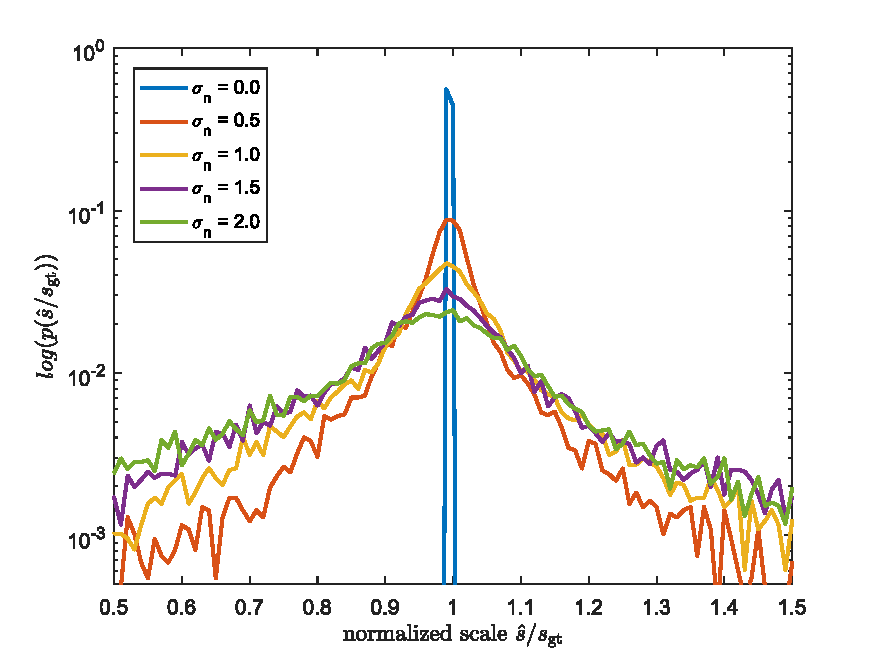
\includegraphics[width=0.5\textwidth]{images/scale_prob_est_e.pdf}
	\caption{}
	\label{experiments:fig:distribution}
\end{figure}
We experiment on a synthetic dataset, with Gaussian-distributed point cloud observed by the pair of pinhole cameras $P_a$ and $P_b$. Both cameras have the resolution 640 by 480 and the focal length 800 pixels. 
Before the cameras are moved, $P_a = \mathrm{I}$. To simulate motion, $P_a$ is moved away from the origin on the surface of a sphere. This generates the cameras as $P_{a'}$ and $P_{b'}$. The direction of motion is random but the distance is neither zero nor far enough to move into the half-sphere opposite to the origin. The principal axis of $P_{a'}$ is ensured to always pass through the center of the sphere. In both cases, $P_b$ maintains a fixed attitude relative to $P_a$. Specifically, it is translated 2 units to the right of $P_a$ on the local x-axis of $P_a$ and rotated 20 degrees around the local z-axis. 

In all tests, both cameras observe a random Gaussian point cloud at the center of the sphere of camera motion. This way there are approximately 100 point correspondences in $P_a$ and $P_{a'}$ and a similar number of correspondences in $P_b$ and $P_{b'}$.

Varying levels of noise between 0 and 2 pixels are added to the points observed in the cameras.  

\subsubsection{Estimate-Distribution Estimate}
Analytically propagating the Gaussian noise through the iterative non-linear essential matrix / relative pose estimator is infeasible. Instead we approximate the distribution through random sampling. We draw $100$ relative pose estimate samples and $\sim 100-500$ second camera correspondences per pose~($\sim 25k$) samples. Specifically we consider the scale estimate quality for each correspondence rather than after 1-pt RANSAC or refinement. 

Figure:~\ref{experiments:fig:distribution} Shows the estimate distribution given varying levels of noise. The figure indicates that the correct answer is the most likely and that any bias is small. This indicates the method should perform well as a initializer for RANSAC-type solvers. 

\subsubsection{Estimate quality given the factor sizes}
\begin{figure}[t]
	\centering
	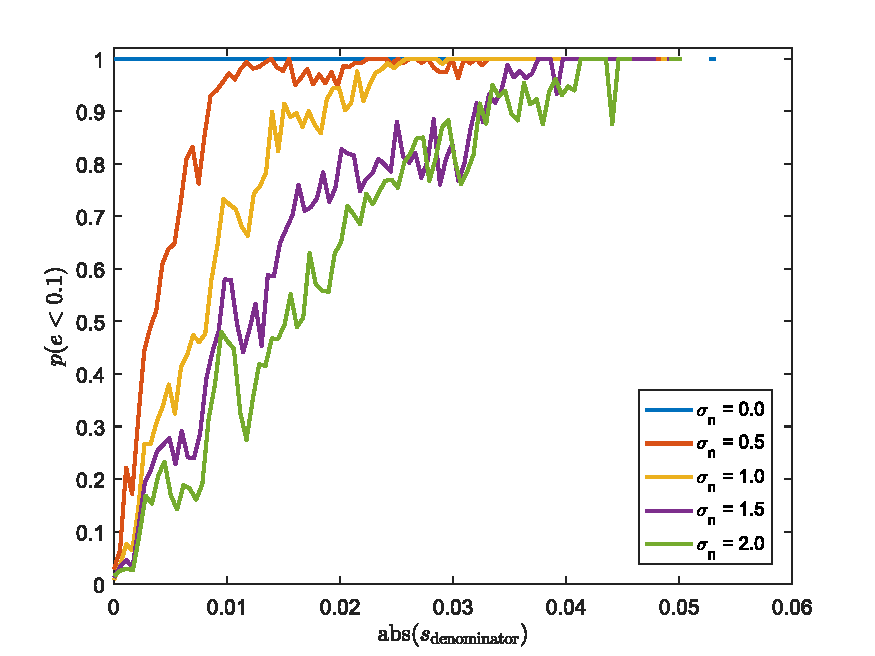
\includegraphics[width=0.5\textwidth]{images/err_prob_denominator_est_e.pdf}
	\caption{}
	\label{experiments:fig:err_prob_denominator}
\end{figure}

\begin{figure}[t]
	\centering
	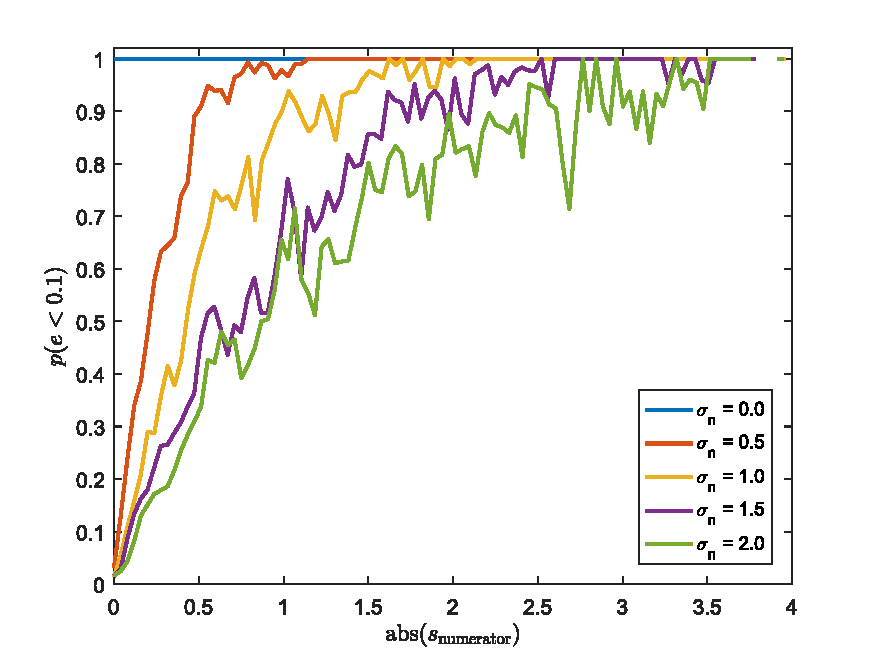
\includegraphics[width=0.5\textwidth]{images/err_prob_numerator_est_e.pdf}
	\caption{}
	\label{experiments:fig:err_prob_numerator}
\end{figure}
Figures~\ref{experiments:fig:err_prob_denominator},~\ref{experiments:fig:err_prob_numerator} validate the hypothesis by showing that with increased values for ($|a|,|b|$) the likelihood of a correct scale estimate is increased and that this effect is stronger with increased noise. The graphs are also sufficient to select a direct threshold based on expected noise statistics. 



\section{Conclusion}
We have presented a re-derivation of the 5+1 point method along with practical details for the effective implementation accompanied by corresponding source code software.
\\ 
\newline
https://github.com/midjji/ssba2016-scale-estimation


% use section* for acknowledgement
\section*{Acknowledgment}
Google for not revealing Clipp et al~\cite{clipp2008robust} until we had had the opportunity to truly understand the method. 

\vspace{2mm} % this command adds a little vertical space to fine-tune
\newpage 
\bibliographystyle{SSBAtrans}
\bibliography{ssba}

% that's all folks
\end{document}
